%%%%%%%%%%%%%%%%%%%%%%%%%%%%%%%%%%%%%%%%%
% Short Sectioned Assignment
% LaTeX Template
% Version 1.0 (5/5/12)
%
% This template has been downloaded from:
% http://www.LaTeXTemplates.com
%
% Original author:
% Frits Wenneker (http://www.howtotex.com)
%
% License:
% CC BY-NC-SA 3.0 (http://creativecommons.org/licenses/by-nc-sa/3.0/)
%
%%%%%%%%%%%%%%%%%%%%%%%%%%%%%%%%%%%%%%%%%

%----------------------------------------------------------------------------------------
%	PACKAGES AND OTHER DOCUMENT CONFIGURATIONS
%----------------------------------------------------------------------------------------

\documentclass[paper=a4, fontsize=11pt]{scrartcl} % A4 paper and 11pt font size
\usepackage{amsmath,amsfonts,graphicx}

\usepackage{booktabs}

\usepackage{listings}
\usepackage{color}
\usepackage{xcolor}
\definecolor{dkgreen}{rgb}{0,0.6,0}
\definecolor{gray}{rgb}{0.5,0.5,0.5}
\definecolor{mauve}{rgb}{0.58,0,0.82}
\lstset{frame=tb,
     %language=Java,
     aboveskip=3mm,
     belowskip=3mm,
     showstringspaces=false,
     columns=flexible,
     basicstyle = \ttfamily\small,
     numbers=none,
     numberstyle=\tiny\color{gray},
     keywordstyle=\color{blue},
     commentstyle=\color{dkgreen},
     stringstyle=\color{mauve},
     breaklines=true,
     breakatwhitespace=true,
     tabsize=3
}

\usepackage[T1]{fontenc} % Use 8-bit encoding that has 256 glyphs
\usepackage{fourier} % Use the Adobe Utopia font for the document - comment this line to return to the LaTeX default
\usepackage[english]{babel} % English language/hyphenation
\usepackage{amsmath,amsfonts,amsthm} % Math packages

\usepackage{lipsum} % Used for inserting dummy 'Lorem ipsum' text into the template

\usepackage{sectsty} % Allows customizing section commands
\allsectionsfont{\centering \normalfont\scshape} % Make all sections centered, the default font and small caps

\usepackage{fancyhdr} % Custom headers and footers
\pagestyle{fancyplain} % Makes all pages in the document conform to the custom headers and footers
\fancyhead{} % No page header - if you want one, create it in the same way as the footers below
\fancyfoot[L]{} % Empty left footer
\fancyfoot[C]{} % Empty center footer
\fancyfoot[R]{\thepage} % Page numbering for right footer
\renewcommand{\headrulewidth}{0pt} % Remove header underlines
\renewcommand{\footrulewidth}{0pt} % Remove footer underlines
\setlength{\headheight}{13.6pt} % Customize the height of the header

\numberwithin{equation}{section} % Number equations within sections (i.e. 1.1, 1.2, 2.1, 2.2 instead of 1, 2, 3, 4)
\numberwithin{figure}{section} % Number figures within sections (i.e. 1.1, 1.2, 2.1, 2.2 instead of 1, 2, 3, 4)
\numberwithin{table}{section} % Number tables within sections (i.e. 1.1, 1.2, 2.1, 2.2 instead of 1, 2, 3, 4)

\setlength\parindent{0pt} % Removes all indentation from paragraphs - comment this line for an assignment with lots of text

%----------------------------------------------------------------------------------------
%	TITLE SECTION
%----------------------------------------------------------------------------------------

\newcommand{\horrule}[1]{\rule{\linewidth}{#1}} % Create horizontal rule command with 1 argument of height

\title{	
\normalfont \normalsize 
\textsc{The University of Melbourne } \\ [25pt] % Your university, school and/or department name(s)
\horrule{0.5pt} \\[0.4cm] % Thin top horizontal rule
\huge COMP90007 Internet Technologies SM2, 2018
Assignment 1 \\ % The assignment title
\horrule{2pt} \\[0.5cm] % Thick bottom horizontal rule
}

\author{Peiyong Wang   (username:PEIYONGW)} % Your name

\date{\normalsize\today} % Today's date or a custom date

\begin{document}

\maketitle % Print the title

%----------------------------------------------------------------------------------------
%	PROBLEM 1
%----------------------------------------------------------------------------------------

\section{Question One}

%\lipsum[2] % Dummy text

\begin{align} 
\begin{split}
bit\;\;rate 	&= baud\;\;rate\times bits\;\;per\;\;baud\\
&=4800\times log_264\\
&=28800\;\;bps\\
\end{split}					
\end{align}

%Phasellus viverra nulla ut metus varius laoreet. Quisque rutrum. Aenean imperdiet. Etiam ultricies nisi vel augue. Curabitur ullamcorper ultricies

%------------------------------------------------

\section{Question Two}

%Lorem ipsum dolor sit amet, consectetuer adipiscing elit. 
%Aenean commodo ligula eget dolor. Aenean massa. Cum sociis natoque penatibus et magnis dis parturient montes, nascetur ridiculus mus. Donec quam felis, ultricies nec, pellentesque eu, pretium quis, sem.

%------------------------------------------------

\begin{align}
	\begin{split}
		total\;\;length\;\;of\;\;heades&=150+100+50\\&=300\;bytes\\	
	\end{split}
\end{align}

\begin{align}
	\begin{split}
		total\;\;length\;\;message&=M+300\;\;bytes\\
	\end{split}
\end{align}

\begin{align}
	\begin{split}
		bandwidth\;\;wasted\;\;on\;\;headers&=\frac{300}{M+300}
	\end{split}
\end{align}

\section{Question Three}
\begin{align}
	total\;\;bits=1280\times720\times3\times8=22118400\;bits
\end{align}
Over a 1-Mbps cable modem:
\begin{align}
	t_1 = \frac{22118400}{1\times 10^6}\approx22.12 s
\end{align}
Over a 100 Mbps ethernet:
\begin{align}
	t_2 = \frac{22118400}{100\times10^6}\approx0.221184s
\end{align}
Over gigabit ethernet:
\begin{align}
	t_3 = \frac{22118400}{1\times10^9}\approx0.02212s
\end{align}

\section{Question Four}
From the information provided by the question, we can have:
\begin{align}
	B=100\;Mbps = 100\times10^6\; bps
\end{align}
\begin{align}
	T_p = \frac{300\;\mu s}{2}=150\;\mu s
\end{align}
and
\begin{align}
	U = \frac{L}{L+2T_pB}=0.4
\end{align}
so we can get:
\begin{align}
	L = 20000\;bits
\end{align}

Hence, the minimum frame size is 20000 bits.


\section{Question Five}

From Figure 5.1 we can clearly see that in the third and fourth column in the green background area are showing the IP address of the source and destination respectively.
\begin{figure}[htbp!]
		\centering
		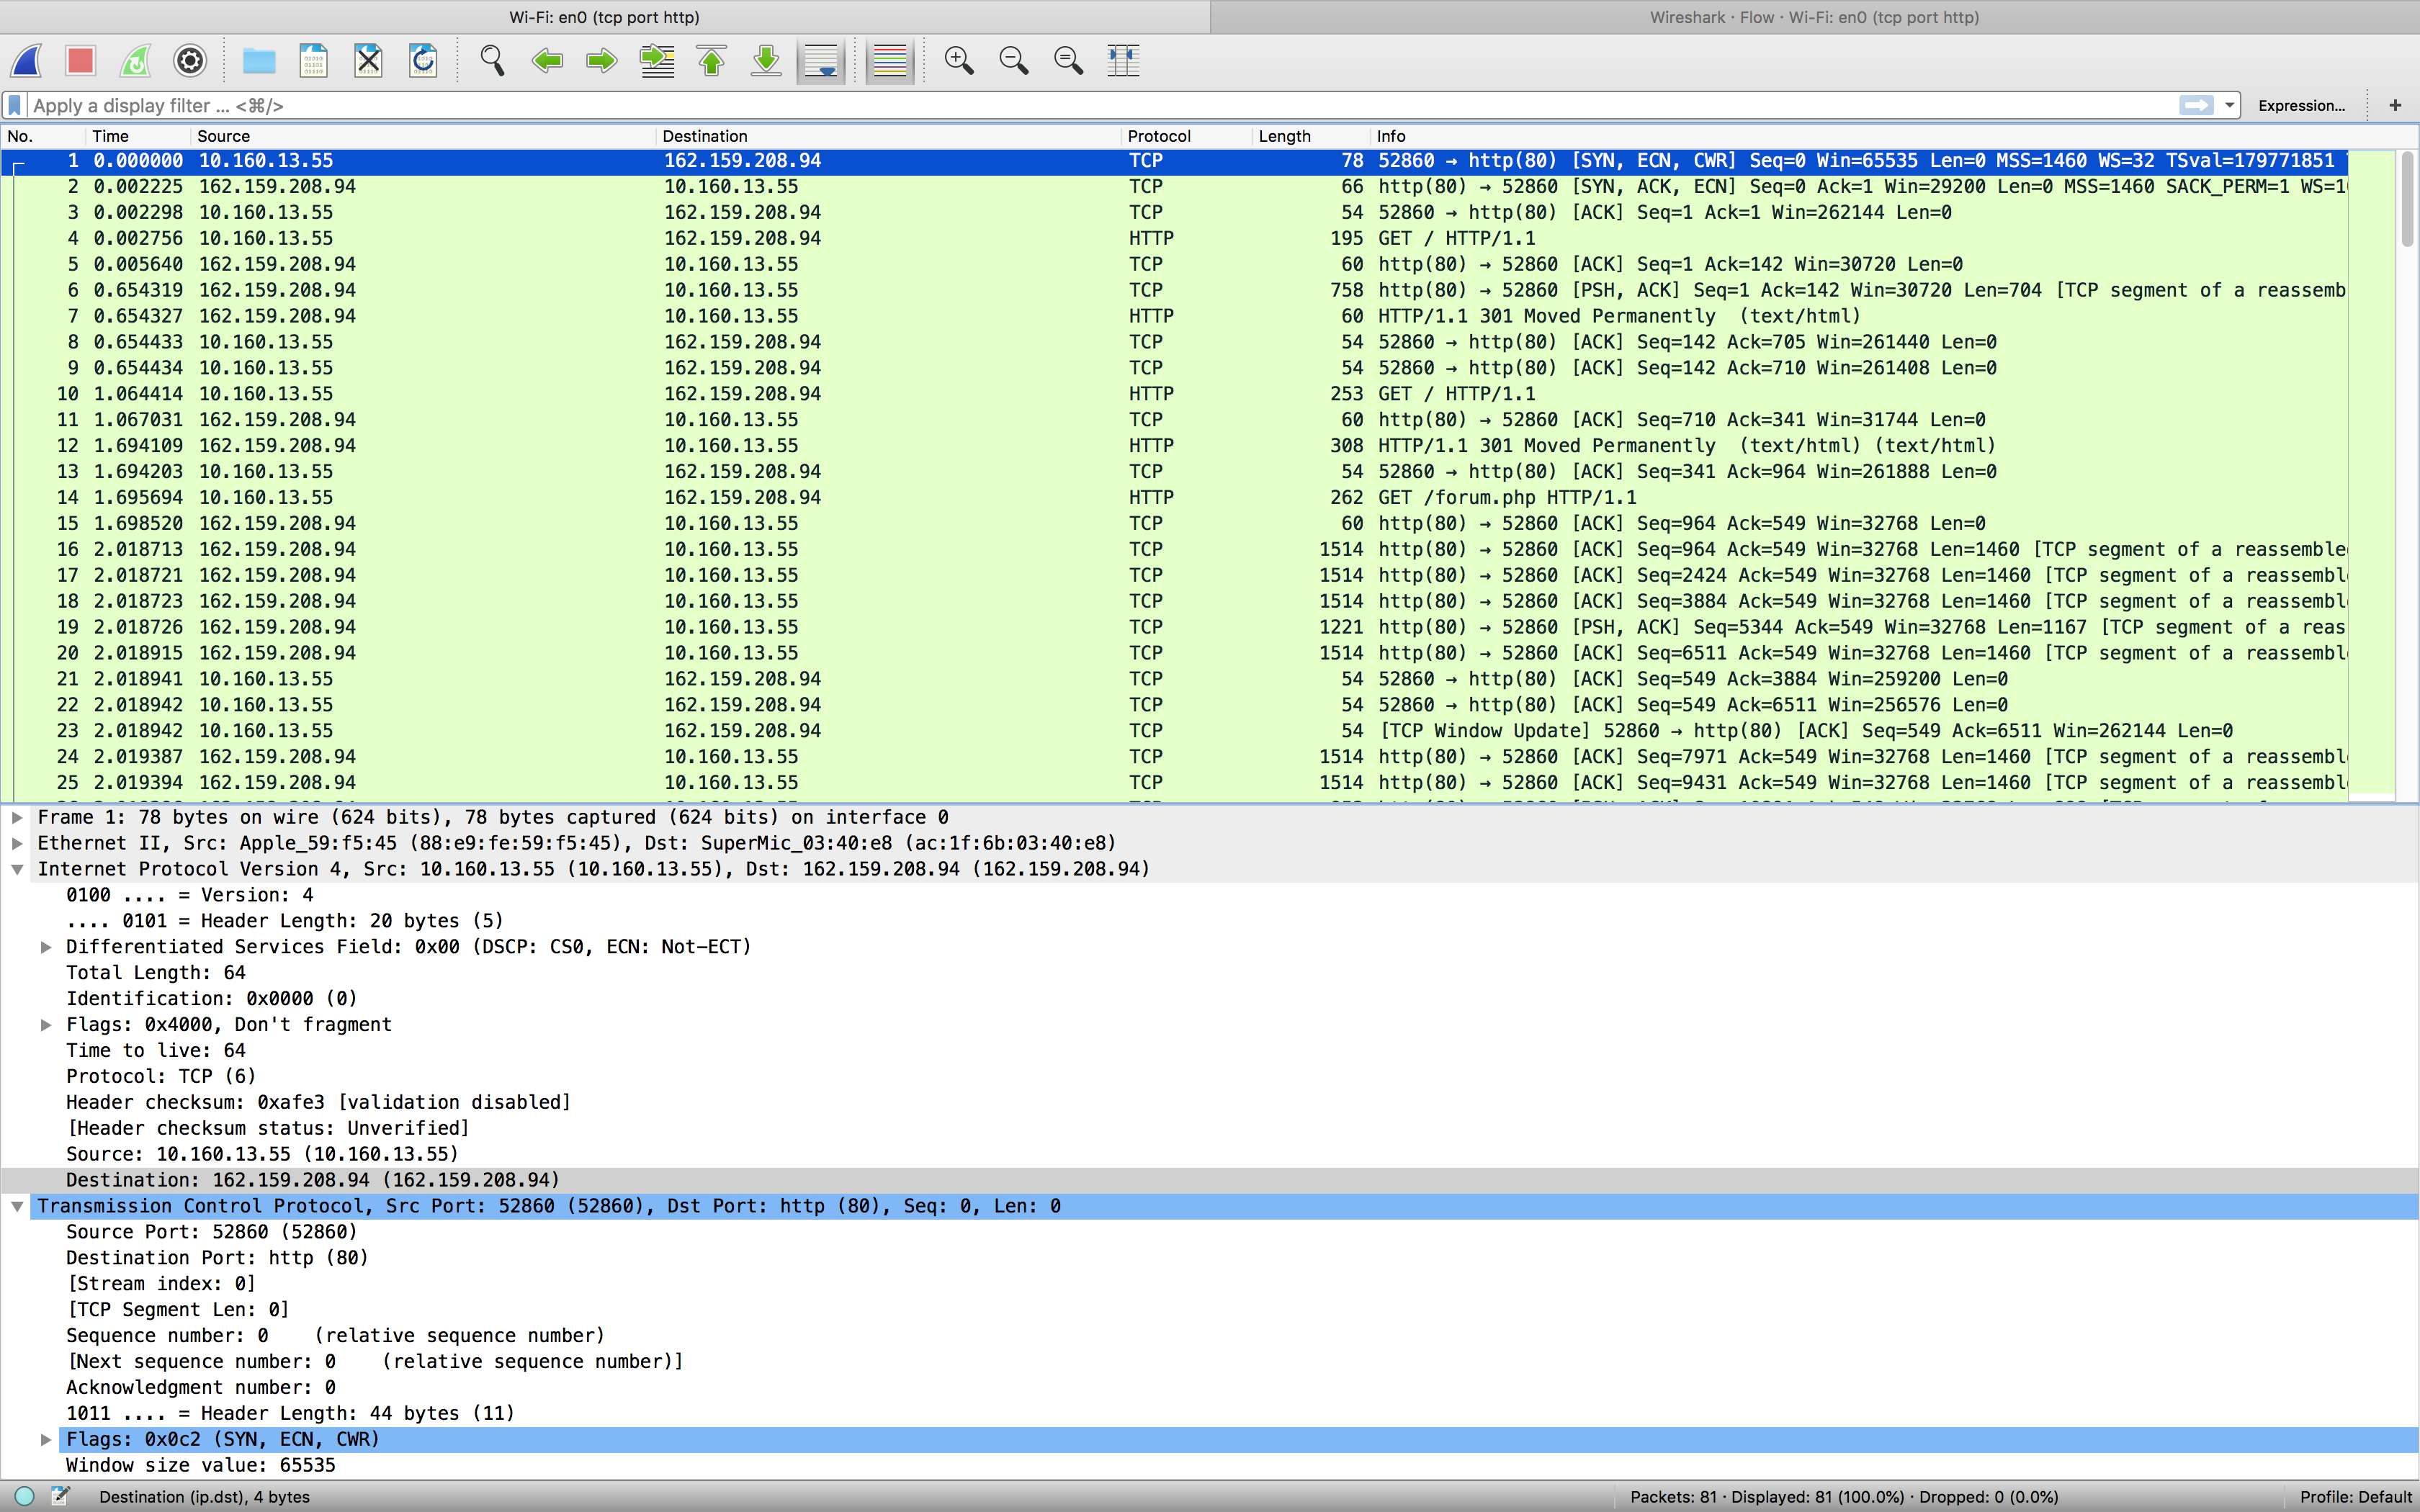
\includegraphics[width=1.0\textwidth]{assigment_1_pics/1}
		\caption{Wireshark trace}%\label{book}
		\vspace{-1em}
\end{figure}



\section{Question Six}
\paragraph{ }

From the flow graph(Fig. 6.2) we can see the essential details of a frame, such as the time of transmission, the size of the frame and the sequence number of the frame and the TCP ports used for the connection. Together with the wireshark trace we can also get the flags,  the window size value and TCP options, etc.
\begin{figure}[htbp!]
		\centering
		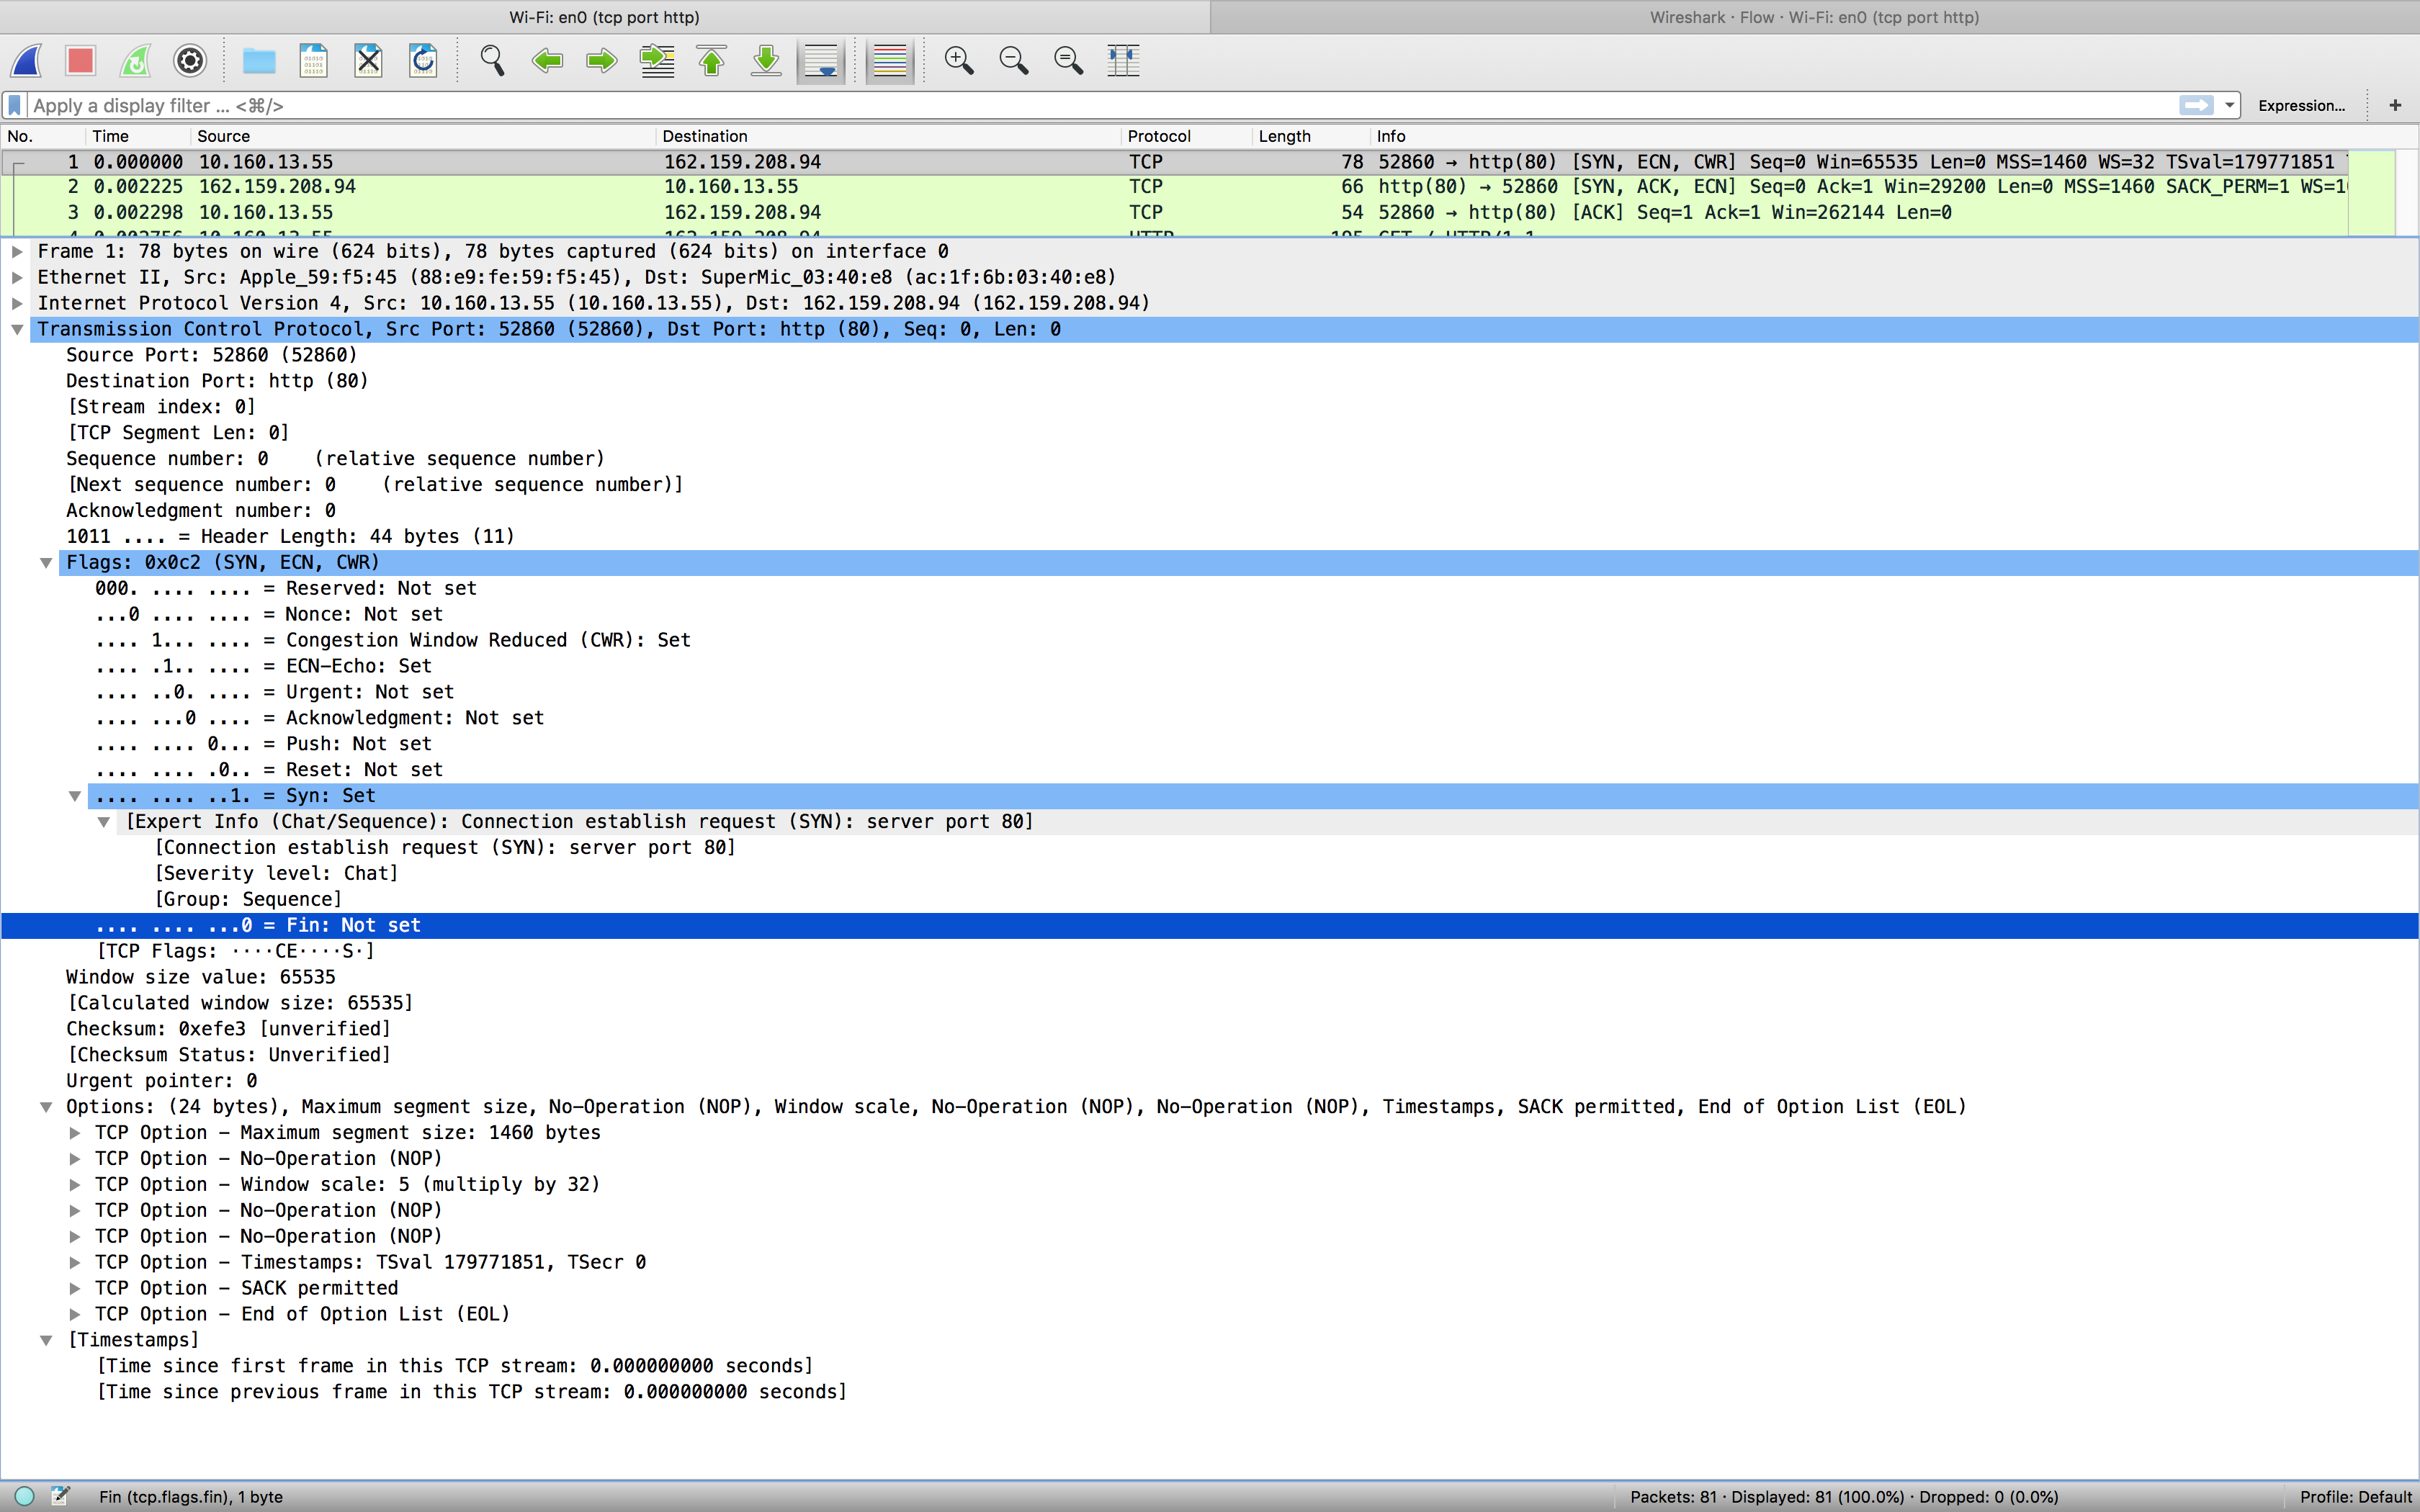
\includegraphics[width=1.0\textwidth]{assigment_1_pics/3}
		\caption{Detailed information for packet 1}%\label{book}
		\vspace{-1em}
\end{figure}

\begin{figure}[htbp!]
		\centering
		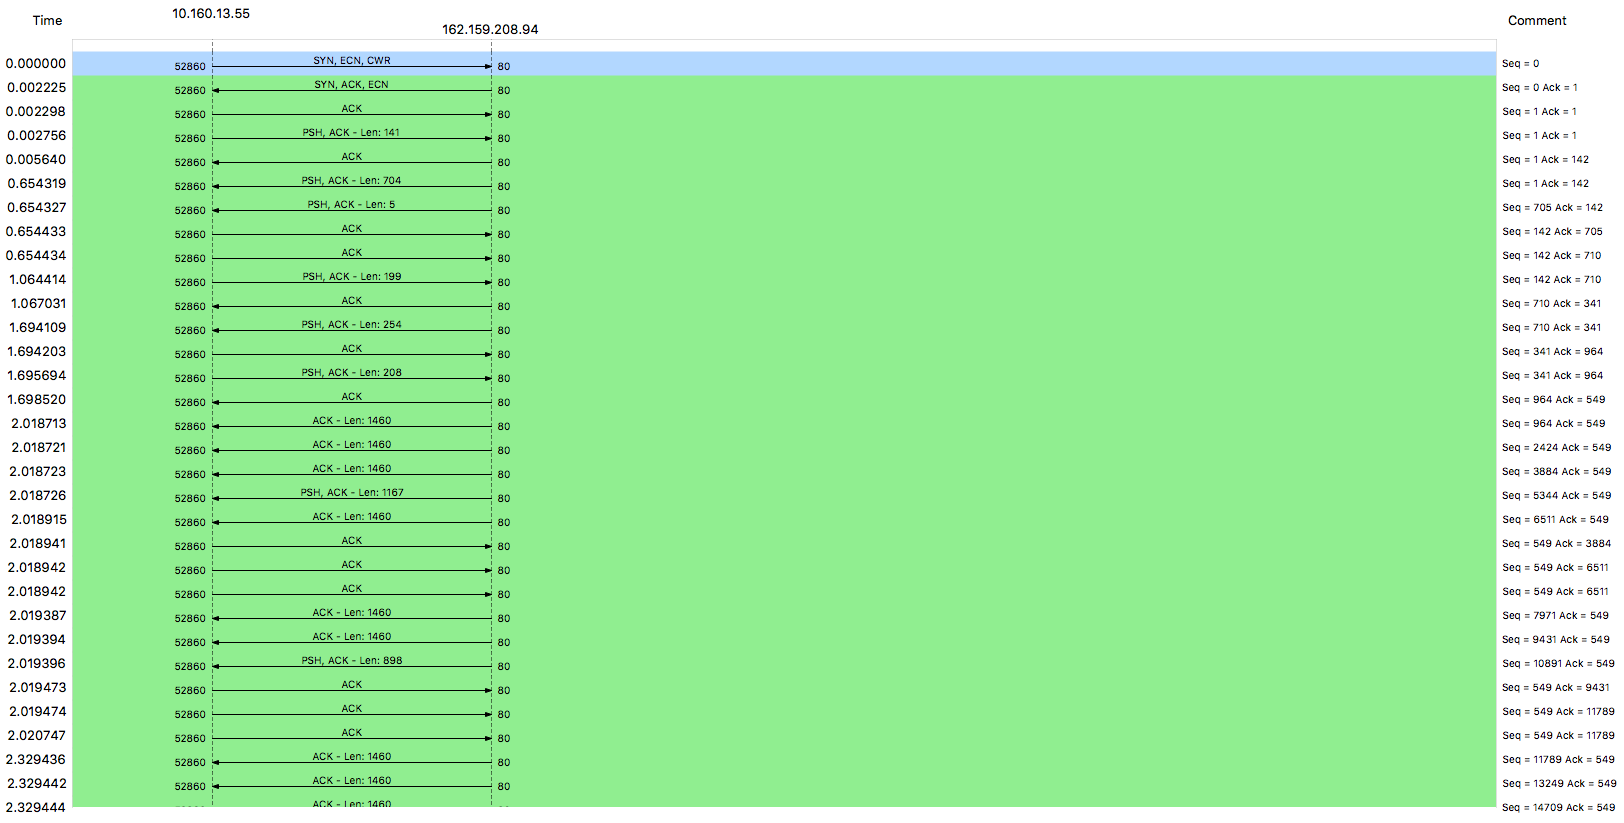
\includegraphics[width=1.0\textwidth]{assigment_1_pics/2}
		\caption{Flow graph}%\label{book}
		\vspace{-1em}
\end{figure}
\paragraph{} 
Also in the figure we can see from Fig 6.2 that there is a three-handshake process when establishing the connection between the source and the destination.



\section{Question Seven }
I believe that this is not a very good approach. Usually, large chunks of data are divided into small packets when being sent through a network. If only an acknowledgement is transmitted to the sender when the whole file is received, when packets lost during the transfer process (even a very small amount of packets are lost), the whole file must be transferred again to the receiver, which is both resource-consuming and time-wasting.

\vbox{}
In my opinion, when large file is divided and sent packet by packet, the receiver should send an acknowledgment with a "packet id code" to tell the sender specifically which packet it received after receiving a packet. So the sender will only need to re-send the lost packets instead of the whole chunk of file, which will save a lot of time and network resources.


%\paragraph{Heading on level 4 (paragraph)}


\section{Question Eight }

\paragraph{I}
This need both large bandwidth and not very high latency. Usually performed by the Australia-Japan Cable and via Internet technologies such as MMCFTP used by a cooperation named Pacific Northwest Gigapop.
\paragraph{II}
This task do not usually require large bandwidth because the game files already installed on the smartphones. However a very low latency (low ping value) network is needed. This is usually satisfied by high speed wifi or 4G mobile networks.
\paragraph{III}
This usually require moderate bandwidth and not very high latency. Internet connections for remote areas used to be provided by dail-up internet. Now they can have broadband network. It is said by news that Amazon is planning to provide Internet access for remote area by drones with wifi transmitter.
\paragraph{IV}
This type of task, such as a fire alarm system, often requires not large bandwidth but very low latency. Technology involved in this field are usually LoRaWAN, NB-IoT, GPRS or even 3/4G.

\paragraph{V}
This requires high bandwidth and low latency often using technologies such as FTP.


\end{document}



%\begin{align} 
%\begin{split}
%(x+y)^3 	&= (x+y)^2(x+y)\\
%&=(x^2+2xy+y^2)(x+y)\\
%&=(x^3+2x^2y+xy^2) + (x^2y+2xy^2+y^3)\\
%&=x^3+3x^2y+3xy^2+y^3
%\end{split}					
%\end{align}





%\begin{tabbing}
%\hspace*{.25in} \= \hspace*{.25in} \= \hspace*{.25in} \= \hspace*{.25in} \= \hspace*{.25in} \=\kill
%\>$Euclid(m,n)=$ \\
%\>\> {\bf while} n$ \neq $ 0 \\
%\>\>\> r $ \leftarrow $ $m$ mod $n$  \\
%\>\>\>  m $\leftarrow$n\\
%\>\>{\bf return} m 
%\end{tabbing}

%Python code:
%\begin{lstlisting}[language = python]
%def gcd(m,n):
%	while n != 0:
%		r = m % n
%		m = n
%		n = r
%	return m
%\end{lstlisting}


%\paragraph{Heading on level 4 (paragraph)}




%\begin{tabbing}
%	\hspace*{.25in} \= \hspace*{.25in} \= \hspace*{.25in} \= \hspace*{.25in} \= \hspace*{.25in} \=\kill
%	{\bf function} find (A,x,n)\\
%	\> j $\leftarrow$ 0\\
%	\> {\bf while} j < n\\
%	\>\> {\bf if} A[j]=x\\
%	\>\>\>  {\bf return} j  \\
%	\>\> j $\leftarrow$ j+1\\
%	\> {\bf return} -1
%\end{tabbing}


%\begin{figure}[htbp!]
%		\centering
%		\includegraphics[width=0.6\textwidth]{lec26.png}
%		\caption{Linked List}%\label{book}
%		\vspace{-1em}
%\end{figure}






%\begin{align}
%A = 
%\begin{bmatrix}
%A_{11} & A_{21} \\
%A_{21} & A_{22}
%\end{bmatrix}
%\end{align}






